\documentclass[12pt]{article}
\usepackage{sydewkrpt}

%%%%%%%%%%%%%%%%%%%%%%%%%%%%
%%%    Begin Document    %%%
%%%%%%%%%%%%%%%%%%%%%%%%%%%%
\begin{document}
\pagenumbering{roman}

\waterlootitle{ME 597: Assignment 1}{

  }{
  Sarah Elliott
  Leigh Pauls\\
  \today
  }

\newpage
\singlespacing
\pagenumbering{arabic}
\section{Bicycle Model}
\setlength{\parindent}{1cm}

The bicycle model has a couple of 



\newpage
\singlespacing
\section{Carrot Planner}
\setlength{\parindent}{1cm}

The robot needs to track a rectangular path. The path \textit{A} is defined by 4 points.
\begin{equation}
\onehalfspacing
\centering
\emph{P =\textnormal{\lbrack} $p_1 p_2 p_3 p_4$ \textnormal{\rbrack} }
\end{equation}
To find the closest point on the path you need to know which part of the path is closest. We can imagine the path as having 4 segments, one for each side of the rectangle. Segment \textit{S($p_n, p_{n+1}$)} is the segment with start and end points at \textit{$p_n$} and \textit{$p_{n+1}$} respectively, where \textit{n = 1, 2, 3}. For each \textit{S}, we need to find the closest point on that segment. Then we will compare the closest points on each segment to see which of the segments is the closest overall. 

Let \textit{$p_{cur}$} be the current point. Let \textit{$r_{p_n/p_{n+1}}$} be the distance between those two points. This notation is extended to all other distances between points. The distance calculation is fairly trivial and not included in this report. Let's define the distance from the first waypoint, \textit{$p_n$}, of the current segment to the closest point on the line as \textit{$d_c$}. 
\begin{equation}
\onehalfspacing
\centering
\emph{$d_c$ = $r_{p_{cur}/p_n}$ * $\frac{r_{p_{n+1}/p_{cur}}^2 -  r_{p_n/p_{cur}}^2 - r_{p_{n+1}/p_n}^2}{-2*r_{p_n/p_cur}*r_{p_{n+1}/p_n}}$ }
%\frac{$r_{p_{cur}/p_{n+1}}^2$ -  $r_{p_{cur}/p_n}^2$ - $r_{p_n/p_{n+1}}^2$}{-2*$r_{p_cur/p_n}$*$r_{p_n/p_{n+1}}$}}
\end{equation}
The figure below shows an example of \textit{$d_c$}. Other point configurations are possible. 
\begin{figure}[ht]
\hspace{0.5cm}
\centering
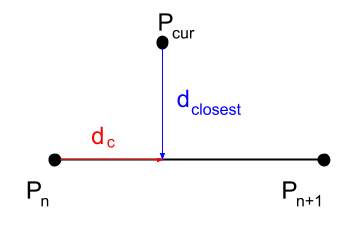
\includegraphics[scale=0.5]{Pictures/points_1.png}
\end{figure}
To find the closest point on the line we have to consider a number of cases. If the points are oriented as above, finding the closest point is fairly straight forward. You just add  \textit{$d_c$} to the location of \textit{$p_n$}. However, what if  \textit{$p_{cur}$} is closest to the top edge of the rectangle and moving counterclockwise? This would mean you need to subtract  \textit{$d_c$} from the location of \textit{$p_n$}. Other cases include if \textit{$d_c$} is negative or greater than \textit{$r_{p_{n+1}/p_n}$}; for example if \textit{$p_{cur}$} is outside the rectangle.

 




\end{document}
